\section{Adrenalingehalt des Blutes}
\begin{code}
	\caption{Skript für die diskrete Berechnung des Verlaufs}
	\mSourceFile{\srcDir/growAdrenalin.m}
	\label{source:2-script}
\end{code}
\begin{figure}[h]
\centering
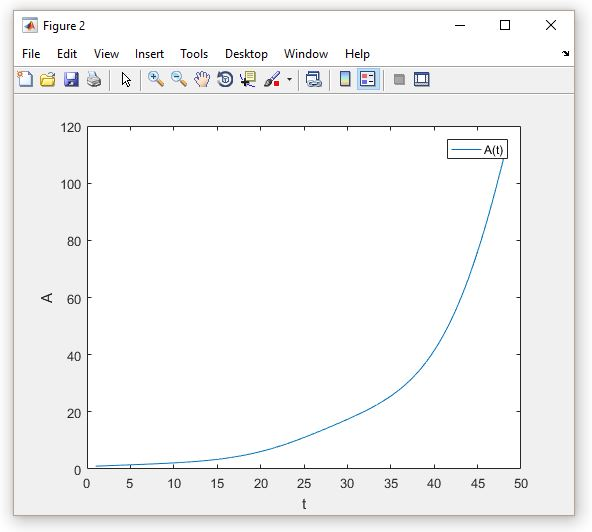
\includegraphics[scale=0.6]{\imageDir/2-test.JPG}
\caption{Verlauf des Adrenalingehalts}
\label{fig:1-c-modell}
\end{figure}
\ \newline
Der Verlauf wurde diskret berechnet, da die Abbaurate proportional zum aktuellen Adrenalingehalt ist.